\documentclass[review]{elsarticle}
\usepackage{lineno,hyperref}
\usepackage{amsmath}
\usepackage{amsfonts}
\usepackage{svg}
\usepackage{tikz}
\usepackage[T1]{fontenc}
\usepackage{graphicx}
\usepackage{caption}
\usepackage{subcaption}
\usepackage{circuitikz}
\usetikzlibrary{positioning}
\modulolinenumbers[5]

\journal{Journal Name}

\bibliographystyle{elsarticle-num}

\newcommand{\vect}[1]{\mathbf{#1}} % vector notation
\newcommand{\mat}[1]{\mathbf{#1}} % matrix notation

\begin{document}
	
	\begin{frontmatter}
		
		\title{Passive and Active Beamforming Optimization in Multi-Cooperative-IRS in Multi-User MISO System}
		
		\author[]{Alireza Tabatabaeian}
		\author[]{Danesh Abdollahi}
		\author[]{Mohammad Sadegh Jafari}
		\author[]{Mohammad Javad Emadi}
		
%		\address[1]{Affiliation 1, Address 1, City 1, Country 1}
%		\address[2]{Affiliation 2, Address 2, City 2, Country 2}
%		\address[3]{Affiliation 2, Address 2, City 2, Country 2}
	
		\begin{abstract}
			This research explores the potential application of Intelligent Reflecting Surfaces (IRS) in the context of future communication networks, specifically focusing on 6G. The study aims to optimize the weighted-sum-rate objective function for a realistic scenario involving two users. In this scenario, the collaboration of two IRS units is considered, with a first-order reflection occurring between them. One of the users experiences an obstacle, highlighting the need for improved network performance.
			To enhance the communication network's performance, a joint optimization approach is employed, optimizing both the passive beamforming coefficients of the IRS and the active beamforming coefficients of the antenna. This optimization is carried out using a coordinate descent algorithm, which iteratively refines the beamforming coefficients to maximize the overall system performance. The research also includes an evaluation of the Signal-to-Interference-plus-Noise Ratio (SINR) improvement in the presence of the first-order reflection between the two IRS units.
			The optimization process comprises several key steps. Firstly, the Lagrangian dual transformation is applied to eliminate the logarithmic function, simplifying the optimization problem. This transformation facilitates a more efficient and tractable optimization process. Additionally, fractional programming techniques are employed to convert fractional terms into linear functions, further streamlining the optimization process. These optimization techniques enable the exploration of optimal beamforming strategies and pave the way for enhanced performance in future wireless communication systems.
		\end{abstract}
		
%		\begin{keyword}
%			intelligent reflecting surfaces optimization\sep 6G networks\sep coordinate descent\sep gradient descent 
%		\end{keyword}
		
	\end{frontmatter}
	
	\linenumbers
	
	\section{Introduction}
			The deployment of intelligent reflecting surfaces (IRS) in wireless communication systems has emerged as a promising technique to enhance the throughput and spectral efficiency. IRSs consist of a large number of reflective elements that can independently control the incident signals, enabling them to manipulate signal propagation. By strategically adjusting the phase shifts of these reflective elements, the IRS can shape the electromagnetic waves and achieve desired signal characteristics. This technology offers significant advantages, such as cost-effectiveness, low power consumption, and easy installation on various infrastructures. The integration of IRSs in 5G and 6G telecommunication wireless networks presents a new frontier in technology materials, revolutionizing the industry. These surfaces can be attached to walls or windows, reflecting unused portions of electromagnetic waves to increase special rates in wireless communication, such as sum-rate or secrecy-rate. Leveraging the capabilities of IRSs, network operators can enhance spectral efficiency, overcome propagation limitations, and meet the demands for higher data rates, improved coverage, and increased network capacity. Continued research and development in IRS technology will unlock even greater opportunities for maximizing the potential of wireless communication systems. $x$ is scalar, $\vect{x}$ is vector, and $\mat{X}$ is matrix. Let $\mat{X}^T$, $\mat{X}^*$, and $\mat{X}^H$ denote the transpose, conjugate, and conjugate transpose of matrix $\mat{X}$, respectively. ${diag} (x_1, \ldots, x_n)$ represents a diagonal matrix with entries $x_1, \ldots, x_n$ on its main diagonal. $\mat{I}_M$ stands for $M \times M$ identity matrix. Operation ${Re}\{\mat{X}\}$ constructs a matrix by extracting the real parts of the entries of matrix $\mat{X}$, while operation $\angle(\mat{X})$ extracts the phases of elements of $\mat{X}$. The modulus of a complex number is denoted by $|\cdot|$, and $j = \sqrt{-1}$ is the imaginary unit. ${C}^{m \times n}$ represents the set of all $m \times n$ complex-valued matrices. The Hadamard product is denoted by $\odot$.\\
	
	\section{System Model and Problem Formulation}
		\begin{figure}[]
			\centering
			\begin{subfigure}{.5\textwidth}
				\flushleft
				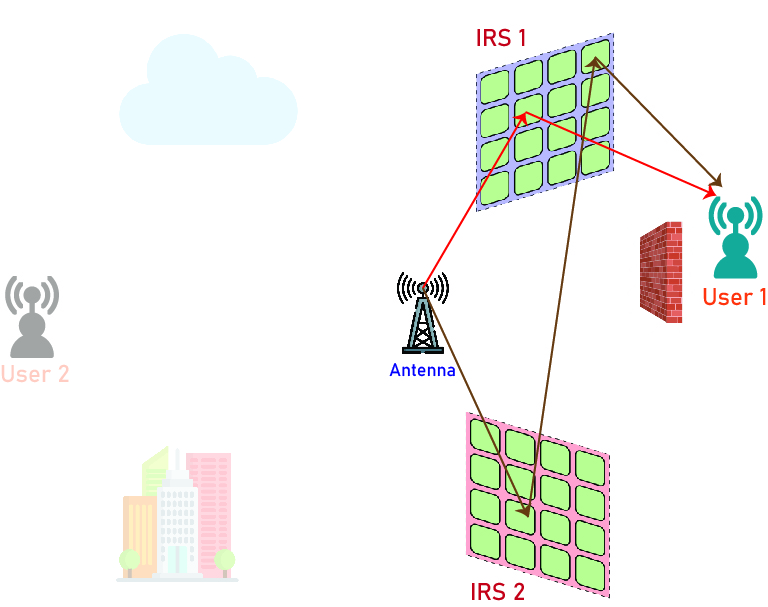
\includegraphics[width=.9\linewidth]{System_Figure2_user1}
				\caption{First User's Links}
				\label{fig:sub2}
			\end{subfigure}%
			\vline
			\begin{subfigure}{.5\textwidth}
				\flushright			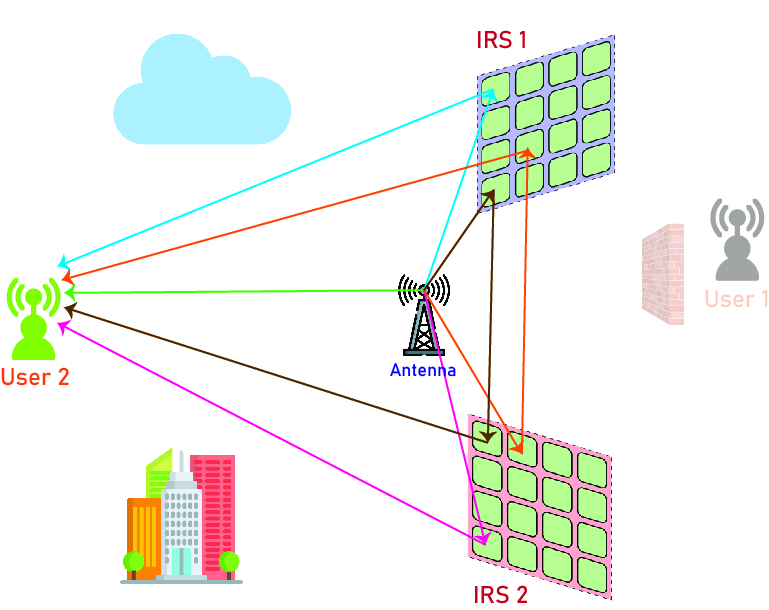
\includegraphics[width=.9\linewidth]{System_Figure2_user2}
				\caption{Second User's Links}
				\label{fig:sub1}
			\end{subfigure}
			\caption{Multi-Cooperative-IRS-aided Multi-User MISO Communication System}
			\label{fig:test}
		\end{figure}
		
		Consider a downlink network consisting of two-cooperative IRS with $M_1$ and $M_2$ elements which has a first-order double reflection between them, a base station with $N_t$ transmit antennas and two users which one of them encountering an obstacle.
		
	\section{Received Signal at User $k$}
		Denote the transmit data symbol to user $k$ by $s_k$. It is assumed that $s_k$ ($k = 1, \ldots, K$) are independent random variables with zero mean and unit variance. Then, the transmitted signal at the BS can be expressed as
		\begin{equation}
			x = \sum_{k=1}^{K} w_k s_k, \label{eq:transmitted_signal}
		\end{equation}
		where $w_k \in \mathbb{C}^{N_t \times 1}$ is the corresponding transmit beamforming vector.
		
		The received signal at user $k$ without considering the obstacles can be expressed as:
		\begin{align*}
			y_k = &\underbrace{h_{d,k}^H x}_
					{\substack{\text{Direct link}}}
				   \quad + \quad \\
    	     	  &\underbrace{h_{r_1,k}^H \Phi_1 G_1 x}_
    	     	  	{\substack{\text{IRS1 link}}}
    	     	   \quad + \quad
   	   			   \underbrace{h_{r_2,k}^H \Phi_2 G_2 x}_
   	   			   	{\substack{\text{IRS2 link}}}
   	   			   \quad + \quad \\ 
    	  		  &\underbrace{h_{r_1,k}^H \Phi_1 D \Phi_2 G_2 x}_
    	  		  	{\substack{\text{Double reflection link}}}
    	  		   \quad + \quad
   	   			   \underbrace{h_{r_2,k}^H \Phi_2 D^H \Phi_1 G_1 x}_
   	   			   	{\substack{\text{Double reflection link}}} \quad + \quad
   	   			   \underbrace{u_k}_
   	   			    {\substack{\text{AWGN}}}
		\end{align*}
	
		where $u_k \sim \mathcal{CN}(0, \sigma_0^2)$ denotes the additive white Gaussian noise (AWGN) at the $k$-th user receiver.
	
	
	\section{Problem Formulation}
		The $k$-th user treats all the signals from other users (i.e.,
		$s_1$, ... , $s_{k-1}$, $s_{k+1}$, ... , $s_K$) as interference. Hence, the decoding SINR of $s_k$ at user $k$ is
		
		\[
			\gamma_k = \frac{{\left|\left(h_{d,k}^H + h_{r_1,k}^H \Phi_1 G_1 + h_{r_2,k}^H \Phi_2 G_2 + h_{r_1,k}^H \Phi_1 D \Phi_2 G_2 + h_{r_2,k}^H \Phi_2 D^H \Phi_1 G_1 \right)w_k\right|^2}}{{\sum_{i=1,i\neq k}^{K} \left|\left(h_{d,k}^H + h_{r_1,k}^H \Phi_1 G_1 + h_{r_2,k}^H \Phi_2 G_2 + h_{r_1,k}^H \Phi_1 D \Phi_2 G_2 + h_{r_2,k}^H \Phi_2 D^H \Phi_1 G_1 \right)w_i\right|^2 + \sigma^2_0}}
		\]
			
		The transmit power constraint of BS is
		
		\[
			\sum_{k=1}^{K} ||w_k||^2 \leq P_T
		\]
		
		Let $\mathbf{W} = [\mathbf{w}_1, \mathbf{w}_2, \ldots, \mathbf{w}_K] \in \mathbb{C}^{N_t \times K}$. In this paper, our objective is to maximize the WSR (Weighted Sum Rate) of all the users by jointly designing the transmit beamforming matrix $\mathbf{W}$ at the base station (BS) and the RC (Reflecting Coefficient) matrix $\Phi_1$ and $\Phi_2$ at the intelligent reflecting surfaces (IRS), subject to the transmit power constraint in $(7)$. The WSR maximization problem is thus formulated as
		
		\begin{align*}
			(P1) \quad \max_{\mathbf{W}, \boldsymbol{\Phi_1}, \boldsymbol{\Phi_2}} \quad & f_1(\mathbf{W}, \boldsymbol{\Phi_1}, \boldsymbol{\Phi_2}) = \sum_{k=1}^{K} \omega_k \log_2(1 + \gamma_k) \\
			\text{s.t.} \quad & \theta_{m_k} \in \mathcal{F}, \quad \forall m_k = 1, \ldots, M_k, \tag{8a} \\
			& \sum_{k=1}^{K} \| \mathbf{w}_k \|_2^2 \leq P_T,
		\end{align*}
	
	\section{Proposed Algorithm}
		According to [], the first problem we must tackle with, is the logarithm function because of the existence of more than one user.
		Consequently, we handle the problem by using Lagrangian dual transform in []:
	
		\[
		f_{1a}(\mathbf{W}, \boldsymbol{\Theta}, \boldsymbol{\alpha}) = \sum_{k=1}^{K} \omega_k \log_2(1 + \alpha_k) - \sum_{k=1}^{K} \omega_k \alpha_k + \sum_{k=1}^{K} \frac{\omega_k (1 + \alpha_k) \gamma_k}{1 + \gamma_k}
		\]
		
		Where $\boldsymbol{\alpha}$ refers to $[\alpha_1, \ldots, \alpha_k, \ldots, \alpha_K]^T$, and $\alpha_k$ is an auxiliary variable for the decoding SINR $\gamma_k$.
		
		In Equation (10), the optimal $\alpha_k$ is given by $\alpha_k^\circ = \gamma_k$.
		
		Then, for a fixed $\boldsymbol{\alpha}$, optimizing $\mathbf{W}$ and $\boldsymbol{\Theta}$ is reduced to:
		
		\[
		(P1'') \quad \max \mathbf{W}, \boldsymbol{\Theta} \quad \sum_{k=1}^{K} \frac{\alpha_k^\sim \gamma_k}{1 + \gamma_k}
		\]
		
		subject to (8a), (8b), where $\alpha_k^\sim = \omega_k(1 + \alpha_k)$.
		
		$(P1'')$ is the sum of multiple-ratio FP problems, and the non-convexity introduced by the ratio operation can be solved via the recently proposed fractional programming technique [22]. In the next two subsections, we will investigate how to solve $\mathbf{W}$ by fixing $\boldsymbol{\Theta}$ and to solve $\boldsymbol{\Theta}$ by fixing $\mathbf{W}$, respectively. Then, the original problem $(P1')$ can be solved in an iterative manner by applying the alternating optimization.
		
		B. Transmit Beamforming
		In this subsection, we investigate how to find a better beamforming matrix $\mathbf{W}$ given fixed $\boldsymbol{\Theta}$ for $(P1'')$. Denote the combined channel for user $k$ by $\mathbf{h}_k = \mathbf{h}_d,k + \mathbf{GH}\boldsymbol{\Theta}\mathbf{h}_r,k$. Then, the SINR $\gamma_k$ in $(6)$ becomes
		\[
		\gamma_k = \frac{{\lVert \mathbf{h}_k \mathbf{w}_k \rVert^2}}{{\sum_{i=1,i\neq k}^{K} \lVert \mathbf{h}_k \mathbf{w}_i \rVert^2 + \sigma_0^2}}
		\]
		Using $\gamma_k$ in $(12)$, the objective function of $(P1'')$ is written as a function of $\mathbf{W}$:
		\[
		f2(\mathbf{W}) = \sum_{k=1}^{K} \frac{\alpha_k^\sim \gamma_k}{{1 + \gamma_k}} = \sum_{k=1}^{K} \frac{\alpha_k}{\alpha_k^\sim} \frac{{\lVert \mathbf{h}_k \mathbf{w}_k \rVert^2}}{{\sum_{i=1}^{K} \lVert \mathbf{h}_k \mathbf{w}_i \rVert^2 + \sigma_0^2}}
		\]
		Thus, given $\boldsymbol{\alpha}$ and $\boldsymbol{\Theta}$, optimizing $\mathbf{W}$ becomes
		\[
		(P2) \quad \max \mathbf{W} \quad f2(\mathbf{W}) \quad \text{s.t.} \quad \sum_{k=1}^{K} \lVert \mathbf{w}_k \rVert^2 \leq PT.
		\]
		It is known that $(P2)$ is the multiple-ratio fractional programming problem. Using the quadratic transform proposed in [22], $f2(\mathbf{W})$ is reformulated as
		\[
		f2a(\mathbf{W}, \boldsymbol{\beta}) = \sum_{k=1}^{K} 2 \sqrt{\alpha_k^\sim} \Re \left\{ \beta_k^* \mathbf{h}_k^H \mathbf{w}_k \right\} - \sum_{k=1}^{K} \lvert \beta_k \rvert^2 \sum_{i=1}^{K} \lVert \mathbf{h}_k \mathbf{w}_i \rVert^2 + \sigma_0^2.
		\]
		where $\boldsymbol{\beta} = [\beta_1, \ldots, \beta_K]^T$, and $\beta_k \in \mathbb{C}$ is the auxiliary variable. Then, based on [22], solving problem $(P2)$ over $\mathbf{W}$ is equivalent to solving the following problem over $\mathbf{W}$ and $\boldsymbol{\beta}$:
		\[
		(P2a) \quad \max \mathbf{W}, \boldsymbol{\beta} \quad f2a(\mathbf{W}, \boldsymbol{\beta}) \quad \text{s.t.} \quad \sum_{k=1}^{K} \lVert \mathbf{w}_k \rVert^2 \leq PT.
		\]
		$(P2a)$ is a biconvex optimization problem, and a common practice for solving it (which does not guarantee global optimality of the solution) is alternatively updating $\mathbf{W}$ and $\boldsymbol{\beta}$ by fixing one of them and solving the corresponding convex optimization problem [38].
		
		Lemma 1: The optimal $\beta_k$ for a given $\mathbf{W}$ is
		\[
		\beta_k^* = \sqrt{\alpha_k^\sim} \frac{{\mathbf{h}_k^H \mathbf{w}_k}}{{\sum_{i=1}^{K} \lVert \mathbf{h}_k \mathbf{w}_i \rVert^2 + \sigma_0^2}}.
		\]
		Then, fixing $\boldsymbol{\beta}$, the optimal $\mathbf{w}_k$ is
		\[
		\mathbf{w}_k^* = \sqrt{\alpha_k^\sim} \beta_k \left( \lambda_0 \mathbf{I}_M + \sum_{i=1}^{K} \lvert \beta_i \rvert^2 \mathbf{h}_i \mathbf{h}_i^H \right)^{-1} \mathbf{h}_k,
		\]
		where $\lambda_0$ is the dual variable introduced for the power constraint, which is optimally determined by
		\[
		\lambda_0^* = \min \left( \lambda_0 \geq 0 : \sum_{k=1}^{K} \lVert \mathbf{w}_k \rVert^2 \leq PT \right).
		\]
		Proof: $\beta_k^*$ in (15) and $\mathbf{w}_k^*$ in (16) can be obtained by setting $\frac{{\partial f2a}}{{\partial \beta_k}}$ and $\frac{{\partial f2a}}{{\partial \mathbf{w}_k}}$ to zero, respectively.
		
		C. Optimizing Reflection Response Matrix $\boldsymbol{\Theta}$
		Finally, we optimize $\boldsymbol{\Theta}$ in $(P1'')$ given fixed $\boldsymbol{\alpha}$ and $\mathbf{W}$.
		Using $\gamma_k$ defined in $(6)$, the objective function of $(P1'')$ is
		expressed as a function of $\boldsymbol{\Theta}$:
		\[
		f3u(\boldsymbol{\Theta}) = \sum_{k=1}^{K} \frac{\alpha_k^\sim \gamma_k}{{1 + \gamma_k}} = \sum_{k=1}^{K} \frac{\alpha_k \lvert ( \mathbf{h}_d,k + \mathbf{h}_r,k\boldsymbol{\Theta}\mathbf{H}_G ) \mathbf{w}_k \rvert^2}{{\sum_{i=1}^{K} \lvert ( \mathbf{h}_d,k + \mathbf{h}_r,k\boldsymbol{\Theta}\mathbf{H}_G ) \mathbf{w}_i \rvert^2 + \sigma_0^2}}.
		\]
		Define $a_{i,k} = \sqrt{\eta} \operatorname{diag}(\mathbf{h}_r,k)\mathbf{G}\mathbf{w}_i$, $b_{i,k} = \mathbf{h}_d,k\mathbf{w}_i$, and $\boldsymbol{\theta} = [\theta_1, \ldots, \theta_N]^T$. Then, $\lvert ( \mathbf{h}_d,k + \mathbf{h}_r,k\boldsymbol{\Theta}\mathbf{H}_G ) \mathbf{w}_i \rvert^2$ in $(19)$ becomes
		\[
		\lvert ( \mathbf{h}_d,k + \mathbf{h}_r,k\boldsymbol{\Theta}\mathbf{H}_G ) \mathbf{w}_i \rvert^2 = \lvert b_{i,k} + \boldsymbol{\theta}^H \mathbf{a}_{i,k} \rvert^2 = \lvert b_{i,k} + \boldsymbol{\theta}^H \mathbf{a}_{i,k} \rvert^2,
		\]
		for all $i$ and $k$. Using $(19)$, $f3u(\boldsymbol{\Theta})$ in $(18)$ is equivalently transformed to a new function of $\boldsymbol{\theta}$:
		\[
		f3(\boldsymbol{\theta}) = \sum_{k=1}^{K} \frac{\alpha_k \lvert b_{k,k} + \boldsymbol{\theta}^H \mathbf{a}_{k,k} \rvert^2}{{\sum_{i=1}^{K} \lvert b_{i,k} + \boldsymbol{\theta}^H \mathbf{a}_{i,k} \rvert^2 + \sigma_0^2}}.
		\]
		Finally, optimizing $\boldsymbol{\Theta}$ is translated to optimizing $\boldsymbol{\theta}$, which is represented as follows:
		\[
		(P3) \quad \max_{\boldsymbol{\theta}} \quad f3(\boldsymbol{\theta}) \quad \text{s.t.} \quad \theta_n \in \mathcal{F}, \forall n = 1, \ldots, N.
		\]
		$(P3)$ is also a multiple-ratio fractional programming problem and can be translated to the following problem based on the quadratic transform proposed in [22]:
		\[
		(P3a) \quad \max_{\boldsymbol{\theta}, \boldsymbol{\epsilon}} \quad f3a(\boldsymbol{\theta}, \boldsymbol{\epsilon}) \quad \text{s.t.} \quad \theta_n \in \mathcal{F}_D, \forall n = 1, \ldots, N,
		\]
		where the new objective function is
		\[
		f3a(\boldsymbol{\theta}, \boldsymbol{\epsilon}) = \sum_{k=1}^{K} \frac{2\sqrt{\alpha_k}\sqrt{\operatorname{Re} \{\epsilon_k^* b_{k,k} + \boldsymbol{\theta}^H \mathbf{a}_{k,k}\}}}{{\sum_{i=1}^{K} \lvert \epsilon_i \rvert^2 \sum_{i=1}^{K} \lvert b_{i,k} + \boldsymbol{\theta}^H \mathbf{a}_{i,k} \rvert^2 + \sigma_0^2}},
		\]
		and $\boldsymbol{\epsilon}$ refers to the auxiliary variable vector $[\epsilon_1, \ldots, \epsilon_K]^T$.
		Similarly, we optimize $\boldsymbol{\theta}$ and $\boldsymbol{\epsilon}$ alternatively. The optimal $\boldsymbol{\epsilon}_k$ for a given $\boldsymbol{\theta}$ can be obtained by setting $\frac{\partial f3a}{\partial \epsilon_k}$ to zero, i.e.,
		\[
		\epsilon_k^* = \sqrt{\alpha_k} \frac{{b_{k,k} + \boldsymbol{\theta}^H \mathbf{a}_{k,k}}}{{\sqrt{\sum_{i=1}^{K} \lvert \epsilon_i \rvert^2 \sum_{i=1}^{K} \lvert b_{i,k} + \boldsymbol{\theta}^H \mathbf{a}_{i,k} \rvert^2 + \sigma_0^2}}}.
		\]
		Then, the remaining problem is optimizing $\boldsymbol{\theta}$ for a given $\boldsymbol{\epsilon}$. It is known that $\lvert b_{i,k} + \boldsymbol{\theta}^H \mathbf{a}_{i,k} \rvert^2$ in $(21)$ can be further written as
		\[
		\lvert b_{i,k} + \boldsymbol{\theta}^H \mathbf{a}_{i,k} \rvert^2 = \boldsymbol{\theta}^H \mathbf{a}_{i,k} \mathbf{a}_{i,k}^H \boldsymbol{\theta} + 2\operatorname{Re} \{ \boldsymbol{\theta}^H \mathbf{a}_{i,k} b_{i,k}^* \} + \lvert b_{i,k} \rvert^2.
		\]
		Substituting $(22)$ and $(23)$ into $(21)$, the optimization problem for $\boldsymbol{\theta}$ is represented as follows:
		\[
		(P4) \quad \max_{\boldsymbol{\theta}} \quad f4(\boldsymbol{\theta}) \quad \text{s.t.} \quad \theta_n \in \mathcal{F}_D, \forall n = 1, \ldots, N,
		\]
		where the objective function is
		\[
		f4(\boldsymbol{\theta}) = f3a(\boldsymbol{\theta}, \boldsymbol{\epsilon}^*) = -\boldsymbol{\theta}^H \mathbf{U} \boldsymbol{\theta} + 2\operatorname{Re} \{ \boldsymbol{\theta}^H \boldsymbol{\nu} \} + C,
		\]
		and
		\[
		\mathbf{U} = \sum_{k=1}^{K} \lvert \epsilon_k \rvert^2 \sum_{i=1}^{K} \mathbf{a}_{i,k} \mathbf{a}_{i,k}^H, \quad \boldsymbol{\nu} = \sum_{k=1}^{K} \sqrt{\alpha_k} \left( \epsilon_k^* \mathbf{a}_{k,k} - \sum_{i=1}^{K} \lvert \epsilon_i \rvert^2 \mathbf{a}_{i,k} b_{i,k}^* \right), \quad C = \sum_{k=1}^{K} \frac{{2\sqrt{\alpha_k} \operatorname{Re} \{\epsilon_k^* b_{k,k}\}}}{{\sigma_0^2 + \sum_{i=1}^{K} \lvert b_{i,k} \rvert^2}}.
		\]
		Since $\mathbf{a}_{i,k} \mathbf{a}_{i,k}^H$ for all $i$ and $k$ are positive-definite matrices, $\mathbf{U}$ is a positive-definite matrix, and $f4(\boldsymbol{\theta})$ is a quadratic concave function of $\boldsymbol{\theta}$. Therefore, the passive beamforming subproblem $(P4)$ is a QCQP, which is the same as that in [16] and [19], and the non-convexity of $(P4)$ is only introduced by the constraint in $(24)$. We will investigate the algorithms to solve $(P4)$ in the next section.
		
		where $p$ and $q$ are auxiliary variables, and the new objective function is given in \cite{ref9}. One can refer to \cite{ref9, Eq. (11)-(12)} to acquire the update rules of $p_k$ and $q_k$. When the auxiliary variables and reflection matrix of IRS are fixed, $W$ is updated by solving
		\[
		\min_{w \in \mathcal{X}_1} f3(W) = f2(\bar{p}, \bar{q}, W, \bar{v}),
		\]
		where $\bar{p}$, $\bar{q}$, and $\bar{v}$ denote the temporal optimization results in the last block. We adopt a variant of the proximal update rule to update $W$ in a closed-form solution. Detailed procedures can be found in \cite{ref9, Eq. (13)-(14)} with extrapolation weight $\epsilon = 0$. Given a fixed $\Phi$, we iteratively update $p$, $q$, and $W$ until the stopping criterion $\epsilon_1$ triggers. These procedures form Step 3 in our general framework.
		
		Given $\bar{p}$, $\bar{q}$, and $\bar{W}$, $v$ is optimized through
		\[
		\min_v f4(v) = v^H Rv - 2\mathrm{Re} \left( v^H e \right),
		\]
		subject to (11a) and (12), where
		\begin{align*}
			R &= \sum_{k=1}^K \left| \bar{q}_k \right|^2 \sum_{i=1}^K \bar{a}_i^k \bar{a}_i^{kH}, \\
			e &= \sum_{k=1}^K p_{\omega_k} (1 + \bar{p}_k) \bar{q}_k^* \bar{a}_k^k - \left| q_k \right|^2 \sum_{i=1}^K \bar{b}_i^k \bar{a}_i^k!,
		\end{align*}
		with $\bar{a}_i^k = H_r^k \bar{w}_i$ and $\bar{b}_i^k = h_d^k \bar{w}_i$. Denote $\Theta = [\theta_1, \theta_2, \ldots, \theta_M]^T$ as expressed in Section II. The gradient is given by
		\[
		\nabla_{\Theta} f4 = 2\mathrm{Re} \left( (Rv - e)^* \odot (-jv) \right),
		\]
		which constitutes Step 4 in Algorithm 1. Overall, we first cyclically update $p$, $q$, and $W$ until convergence, and then use the gradient information (13) to update $\Phi$.
		
	\section{SIMULATION RESULTS}
	
	The results of the research should be presented in this section. It should include tables, figures, and other relevant visualizations.
	
	\section{CONCLUSIONS}
	
	In this section, the results of the research should be discussed and interpreted. Any implications and limitations of the research should also be discussed.
	
	\section{APPENDIX}
	
	The conclusion should summarize the main findings of the research and its significance. It should also include any recommendations for future research.
	
	\section*{REFERENCES}
	
	\bibliography{references}
	
\end{document}
